\chapter{\uppercase{Programació}}
% Testejar cosetes i poder treure algun screenshot (?, o l'screen shot no fa falta?
% Adjuntar codi, aquí o en annex
Tot el hardware explicat anteriorment ha d'anar recolzat del seu software. En aquest cas, el més primordial és mostrejar la senyal analògica per tal de poder determinar si aquesta supera un llindar de màxim o si disminueix d'un llindar de mínim. Això ho fa l'Arduino Nano, la qual disposa d'entrades analògiques.\\
\newline En segon lloc cal que l'Arduino Nano controli els LEDs i n'encengui més o menys en funció de la freqüència cardíaca mesurada.\\
\newline Mostrar la pàgina web se n'encarrega l'ESP-01, i hem comprovat que requereix d'uns 100 ms per fer-ho. La resta del temps es dedica a sol·licitar dades a l'Arduino Nano. Si aquesta no té cap nova dada de freqüència cardíaca per enviar, simplement no diu res. 


\section{Organigrama Arduino Nano}
L'organigrama de la Figura \ref{fig:organigrama2} ens permet entendre a alt nivell el funcionament del programa que s'encarrega de llegir la tensió analògica provinent de l'ADS8232, calcular la freqüència cardíaca, controlar els LEDs i passar la freqüència cardíaca. A l'annex de programa figura el codi complet.


% fill=blue!20, 
\tikzstyle{decision} = [diamond, draw, fill=orange!30, 
    text width=4.5em, text badly centered, node distance=3cm, inner sep=0pt]
\tikzstyle{block} = [rectangle, draw, fill=blue!20, 
    text width=5em, text centered, rounded corners, minimum height=4em]
\tikzstyle{line} = [draw, -latex']
\tikzstyle{cloud} = [draw, ellipse,fill=red!20, node distance=3cm,
    minimum height=2em]
    
\begin{figure}[H]
\begin{center}
\begin{tikzpicture}[node distance = 3cm, auto, scale=0.8, every node/.style={scale=0.8}]
    % Place nodes
    \node [block] (inici) {\footnotesize Inicialització};
    \node [block, text width=4cm, minimum height = 1cm, inner sep=0pt, below of=inici, node distance=2.5cm] (lectura) {\footnotesize Lectura entrada analògica};
 \node [decision, right of=lectura, node distance=4cm] (max) {\footnotesize $Lectura > llindar\_max ?$};
 \node [decision, left of=lectura, node distance=4cm] (min) {\footnotesize $Lectura < llindar\_min ?$};  
    \node [block, below of=max, minimum height = 1cm, inner sep=0pt, minimum width=5cm, text width=5cm, node distance=3cm] (bloc_max) {\footnotesize $memoria\_temps = millis();$   $flag = 1;$};  
    \node [block, minimum width=5cm, text width=4.5cm, minimum height = 1cm, inner sep=0pt, below of=bloc_max, node distance=2cm] (accio_pic) {\footnotesize $calcul\_bpm(); disponible = 1;$};    
    \node [block, node distance=2cm, minimum width=5cm, text width=4.5cm, minimum height = 1cm, inner sep=0pt, below of=accio_pic, node distance=2cm] (apaga) {\footnotesize Apaga LEDs}; 
        
    \node [block, minimum width=5cm, text width=4.5cm, minimum height = 1cm, inner sep=0pt, below of=min, node distance=3cm] (bloc_min) {\footnotesize $flag = 0;$}; 
    
\node [block, node distance=6cm, minimum width=5cm, text width=4.5cm, minimum height = 1cm, inner sep=0pt, below of=bloc_min] (leds) {\footnotesize $Encendre \ LED == true \ ? \ encen\_LED :$}; 
    
   %Encendre LED == true ? encen_LED :
    
%        \node [ left of=wifi, node distance=4cm] (punt) {.};

    % Draw edges
    \path [line] (inici) -- (lectura);
    \path [line] (lectura) -- (max);
    \path [line] (lectura) -- (min);
    
    \path [line] (max) -- (bloc_max);
    \path [line] (bloc_max) -- (accio_pic);
    \path [line] (accio_pic) -- (apaga);
    
    \path [line] (min) -- (bloc_min);
    
    \path [line] (bloc_min) -- (leds);
    \path [line] (apaga) -- (leds);

     \draw [->] (leds) to[out=170, in=135] node[auto] {} (inici);
\end{tikzpicture}
\end{center}
\caption{Organigrama del codi}
\label{fig:organigrama2}
\end{figure}

\noindent Després de cada petició de la placa ESP-01 a l'Arduino, per I2C, s'executa una rutina d'interrupció que envia per I2C la freqüència cardíaca si encara no l'ha enviat. Si l'ha enviat no envia res.

%\section{Explicació}
%
\section{Programació Arduino Nano}
Tot el codi figura a l'annex. Creiem, però, que és important comentar aquells aspectes o fragments més importants.\\
\newline Definim un color per cada LED de l'anell de LEDs i ho guardem en un vector.
\end{spacing}
\begin{spacing}{1}
\begin{lstlisting}[style=myArduino]
int32_t c0 = strip.Color(255, 255, 0);
uint32_t c1 = strip.Color(178, 255, 0);
uint32_t c2 = strip.Color(55, 255, 0);
uint32_t c3 = strip.Color(6, 172, 38);
uint32_t c4 = strip.Color(0, 210, 255);
uint32_t c5 = strip.Color(8, 0, 255);
uint32_t c6 = strip.Color(1, 0, 255);
uint32_t c7 = strip.Color(107, 0, 222);
uint32_t c8 = strip.Color(101, 0, 144);
uint32_t c9 = strip.Color(255, 0, 208);
uint32_t c10 = strip.Color(255, 0, 199);
uint32_t c11 = strip.Color(123, 0, 96);
uint32_t c12 = strip.Color(128, 0, 46);
uint32_t c13 = strip.Color(223, 2, 10);
uint32_t c14 = strip.Color(223, 0, 0);
uint32_t c15 = strip.Color(255, 0, 0);
uint32_t leds[16]={c0, c1, c2, c3, c4, c5, c6, c7, c8, c9, c10, c11, c12, c13, c14, c15};
\end{lstlisting}

\end{spacing}
\begin{spacing}{1.5}
%
\noindent Al \textbf{void setup()} definim l'adreça I2C que volem que tingui el dispositiu, en aquest cas hem escollit l'adreça 0x08.
\end{spacing}
\begin{spacing}{1}
\begin{lstlisting}[style=myArduino]
void setup() {
  Wire.begin(8);  //0x08=8, adreça que fem servir per comunicar amb l'ESP-01
//  Wire.onReceive(receiveEvent);
  Wire.onRequest(sendEvent);
  ...
}
\end{lstlisting}
\end{spacing}
\begin{spacing}{1.5}
%
\noindent Al \textbf{void loop()} ens dediquem a llegir molt ràpidament la tensió analògica que ens arriba del sensor de freqüència cardíaca. Prèviament s'han definit dos llindars, un de mínim i un de màxim, que permeten identificar de forma correcta i robusta els pics, amb els quals es calcula la freqüència cardíaca en batecs per minut (bpm).\\
\newline Per determinar si cal encendre LEDs o no es mira la freqüència cardíaca mesurada i el temps respecte l'última encesa de LEDs. Això ho fem per aconseguir un efecte d'encesa gradual, enlloc de veure com de cop s'encenen tots els LEDs.
\end{spacing}
\begin{spacing}{1}
\begin{lstlisting}[style=myArduino]
  // Determinem si cal encendre leds o no
    if ((millis()-temps_memoria_2) > delay_entre_leds)
    {
      if (i<freq_bpm*16/130)
      {
       strip.setPixelColor(i, leds[i]);
       strip.show();
      i++;      
      }
      temps_memoria_2 = millis();
    }
\end{lstlisting}
\end{spacing}
\begin{spacing}{1.5}
%
\noindent Per últim, definim una funció que s'encarrega de contestar amb la dada de freqüència cardíaca més recent, sempre que no l'hagi enviat prèviament.
\end{spacing}
\begin{spacing}{1}
\begin{lstlisting}[style=myArduino]
// Envia la frequencia enlloc d'un numero random, i com a condicional té un boolea que diu si cal enviar o no
void sendEvent(int howmany){
  // Funció per respondre per I2C a l'ESP-01
  /*
  randNumber = random(40, 200); // Serial.print("generat: "); Serial.println(randNumber);
  
  cadena[2] = (randNumber - (randNumber/10)*10) + 48; 
  cadena[1] = (randNumber/10 - (randNumber/100)*10) + 48; 
  cadena[0] = (randNumber / 100) + 48; 
  // Serial.println(cadena);

  if (randNumber >= 40){
    Wire.write(cadena); // Serial.println("major de 100");
  }
 //  Wire.endTransmission(true);
 // Wire.write(cadena); // 3 bytes
 */
  
  cadena[2] = (freq_bpm - (freq_bpm/10)*10) + 48; 
  cadena[1] = (freq_bpm/10 - (freq_bpm/100)*10) + 48; 
  cadena[0] = (freq_bpm / 100) + 48; 
  if (dada_enviada == 0){
    Wire.write(cadena);
    dada_enviada = 1;
  }

}
\end{lstlisting}
\end{spacing}
\begin{spacing}{1.5} 

\section{Organigrama placa Wi-Fi}
L'organigrama de la Figura \ref{fig:organigrama} és una forma simplificada d'explicar com s'ha programat l'ESP-01. A l'annex de programa figura el codi complet.


% fill=blue!20, 
\tikzstyle{decision} = [diamond, draw, fill=orange!30, 
    text width=4.5em, text badly centered, node distance=3cm, inner sep=0pt]
\tikzstyle{block} = [rectangle, draw, fill=blue!20, 
    text width=5em, text centered, rounded corners, minimum height=4em]
\tikzstyle{line} = [draw, -latex']
\tikzstyle{cloud} = [draw, ellipse,fill=red!20, node distance=3cm,
    minimum height=2em]
    
\begin{figure}[H]
\begin{center}
\begin{tikzpicture}[node distance = 2cm, auto, scale=0.65, every node/.style={scale=0.65}]
    % Place nodes
    \node [block] (inici) {Inicialització};
    \node [block, below of=inici, node distance=2cm] (intent) {Intenta connexió Wi-Fi};
    \node [decision, below of=intent] (decide) {Dispositiu connectat via Wi-Fi?};
    \node [block, left of=decide, node distance=4cm] (delay) {Espera 500 ms};
        \node [decision, below of=decide, node distance=4cm] (wifii) {Client connectat?};
            \node [block, below of= wifii, node distance=3cm] (comprova) {Sol·licita dada};
            \node [block, right of=wifii, node distance=4cm] (webbb) {Mostra web};
    \node [decision, below of=comprova, node distance=3cm] (mesura) {Dada vàlida?};
    \node [decision, below of=mesura, node distance=4cm] (wifi) {Client connectat?};
    \node [block, right of=wifi, node distance=4cm] (guarda) {Guarda dada};
    \node [block, below of=wifi, node distance=3cm] (webb) {Mostra web};
    
        \node [ left of=wifi, node distance=4cm] (punt) {.};

    % Draw edges
    \path [line] (inici) -- (intent);
    \path [line] (intent) -- (decide);    
    \path [line] (decide) -- node [near start] {Sí}(wifii);    
    \path [line] (decide) -- node [near start] {No}(delay);
    

    \path [line] (comprova) -- (mesura); 
    \path [line] (mesura) -- node [near start] {No} (wifi); 
	\path [line] (mesura) -| node [near start] {Sí} (guarda);
	\path [line] (guarda) -- (wifi);
   \path [line] (wifi) -- node [near start] {Sí} (webb);
   
   \path [line] (webb) -| (punt);
   \path [line] (wifii) -- node [near start] {Sí} (webbb);
    \path [line] (wifii) -- node [near start] {No} (comprova);
 \path [line] (webbb) |-  (comprova);    
    
	\path [line] (wifi) -- node [near start] {No} (punt);
	\path [line] (punt) |- (comprova);   
	
    \path [line] (delay) |- (intent);
    
    
\end{tikzpicture}
\end{center}
\caption{Organigrama del codi}
\label{fig:organigrama}
\end{figure}

%\section{Explicació}
%
\section{Programació placa Wi-Fi}

\noindent Quan s'inicia el programa el primer que es fa és inicialitzar variables i intentar connectar-se a la xarxa Wi-Fi de la qual s'ha definit la contrasenya i el nom, o més ben dit, l'SSID. Si el dispositiu és incapaç de connectar-se a la xarxa Wi-Fi ho segueix intentant cada mig segon.
\end{spacing}
\begin{spacing}{1}
\begin{lstlisting}[style=myArduino]
  // Ens connectem al Wi-Fi amb l'adreça i la contrasenya definits
  Serial.print("Connectant a: ");
  Serial.println(ssid); // Mostrem l'adreça del Wi-Fi
  WiFi.begin(ssid, password); // Iniciem la comunicació
  
  while (WiFi.status() != WL_CONNECTED) {
    delay(500);
    Serial.print("."); // Cada 0,5 s que passin sense connectar-se mostra un punt
  }
  
  // S'ha connectat
  Serial.println("");
  Serial.println("WiFi connectat");
  Serial.println("Adreça IP: ");
  Serial.println(WiFi.localIP());
  server.begin();
\end{lstlisting}

\end{spacing}
\begin{spacing}{1.5}

\noindent Un cop té connectivitat Wi-Fi mira si té algun client connectat, i en cas de què sigui així li mostra la web.\\
\newline Per defecte s'han emplenat els vectors de dades fictícies per tal de mostrar com es presenten les gràfiques que es fan amb JavaScript. A mesura que passin les hores aquestes dades s'aniran sobreescrivint per dades reals. La resta de la pàgina web està definida amb etiquetes HTML.\\
\newline Per escriure les dades es recorren els vectors. Per una mateixa fila es miren totes les columnes, després es passa a la següent fila.
\end{spacing}
\begin{spacing}{1}
\begin{lstlisting}[style=myArduino]
            client.println("data.addRows([\n"); 
            for (i = 0; i < files; i++) { // i = hora_actual ...
              client.println("[");
              client.println(String(vector2[i][0]));
              for (j = 1; j < 3; j++) {
                client.println(","); client.println(String(vector2[i][j]));
              }
              client.println("]"); client.println(","); client.println("\n");
            }
\end{lstlisting}

\end{spacing}
\begin{spacing}{1.5}
%
\noindent Per tal de sol·licitar la freqüència cardíaca per I2C el que es fa és plantejar una funció anomenada \textbf{demana\_dada()} que demana 3 bytes i si la dada és vàlida la guarda en memòria. A més, també s'encarrega de calcular la variància de les dades del primer vector, calcula la mitjana de freqüència cardíaca d'aquella hora i fa un calcula aproximat de la variància d'aquella hora. D'aquesta manera es preparen les dades per la pàgina web.
\end{spacing}
\begin{spacing}{1}
\begin{lstlisting}[style=myArduino]
void demana_dada (){
  Wire.requestFrom(8, 3); //0x08 = 8;

  while (0 < Wire.available()) {
    char c = Wire.read(); 
    int nombre = c-48; 
    //  Serial.println(nombre);
    n_rebut = n_rebut*10 + (c-48);
  }

  if (n_rebut != -2523 && n_rebut != 0){
  
      vector[i_fila][0] = millis()/1000.0;
      vector[i_fila][1] = n_rebut;
      
          for (i=0; i<files; i++){
            mitjana = vector[i][1]*(1.0/(i+1.0)) + mitjana*i/(i+1.0);  
          }
          int sumatori = 0;
          for (i=0; i<files; i++){
            sumatori += (mitjana - vector[i][1]) * (mitjana - vector[i][1]);  
          }
          desvest = sumatori / (files-1);
  
      vector[i_fila][2] = 1.0*pow(desvest, 0.5);
    // 2 ms per fer els càlculs de mitjana i desvest, acceptable  
          
      i_fila++;
      if (i_fila > files) {
        i_fila = 0;
      }
   
      Serial.println(n_rebut);  
  
  //----- dades hora, 2a gràfica -----
  
      n_dades_hora++;
      vector2[hora_actual][0] = hora_actual;
      vector2[hora_actual][1] = n_rebut*1.0/(n_dades_hora) + vector[hora_actual][1]*(n_dades_hora-1)/(n_dades_hora);
      vector2[hora_actual][2] = vector[i_fila-1][2]*1.0/(n_dades_hora) + vector2[hora_actual][2]*(n_dades_hora-1)/(n_dades_hora);
  }
    
  else {
      Serial.println("és -2523"); // l'Arduino Nano no té cap dada nova, captem aquest número
  }

    n_rebut = 0;
    Wire.endTransmission(); // Afegit, no fa cap mal
}
\end{lstlisting}
\end{spacing}
\begin{spacing}{1.5}
%
\noindent Cada poc més de 50 ms es crida aquesta funció. La freqüència amb què es crida aquesta funció és més que suficient per poder garantir que no ens perdem cap dada de freqüència cardíaca, ja que el període d'un cor en repòs és de l'ordre de 1 s. Si algú té el cor molt accelerat, per exemple 120 bpm, això són 500 ms de període.

\section{Pàgina web}
\noindent A continuació es poden observar algunes captures de la pàgina web creada. A cada figura es mostren dues gràfiques, cada una és d'una branca i mostra la tensió de les 5 plaques que té connectades.\\
\newline Quan s'entra a la web el primer que es veu és el que detalla la Figura \ref{fig:1}.

\begin{figure}[H]
\begin{center}
\fbox{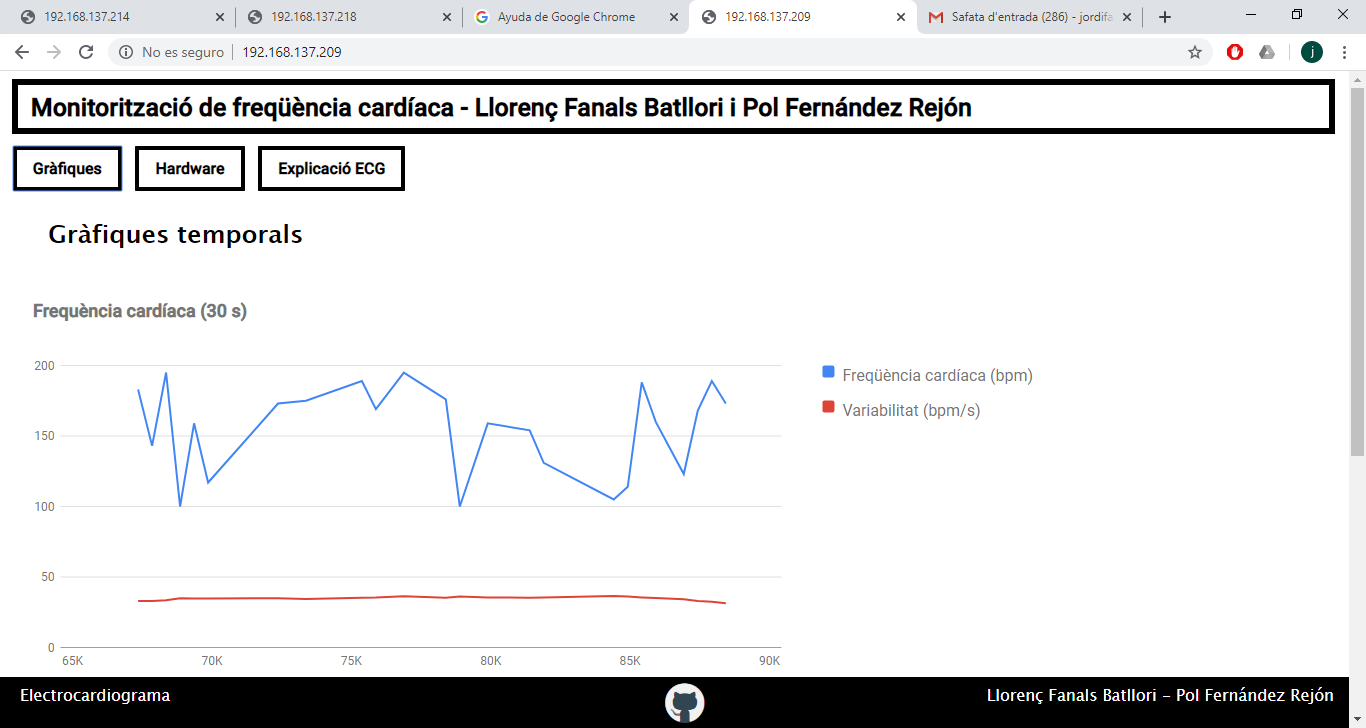
\includegraphics[scale=0.43]{images/web_ecg.png}}
\end{center}
\caption{Gràfica de les dades més recents, web}
\label{fig:1}
\end{figure}

\noindent \\ El fet d'utilitzar JavaScript permet inserir contingut dinàmic. Al passar el ratolí per sobre una línia es ressalta la línia i els punts que la formen. És possible visualitzar el valor de cada punt col·locant el ratolí sobre seu A la Figura \ref{fig:2} s'aprecia.
\begin{figure}[H]
\begin{center}
\fbox{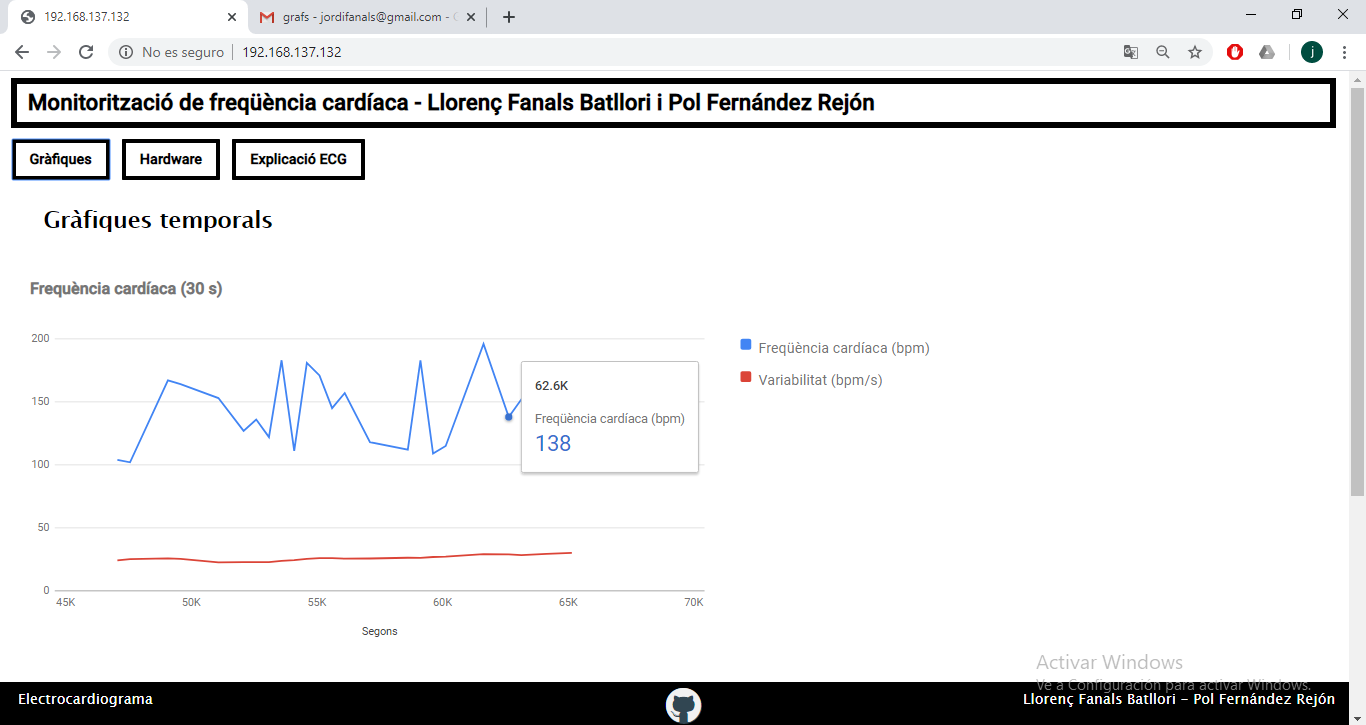
\includegraphics[scale=0.43]{images/web_punt.png}}
\end{center}
\caption{Gràfica ressaltant el valor d'un punt}
\label{fig:2}
\end{figure}

\noindent \\ Es pot navegar pels menús per veure un contingut o altre. Per exemple, podem demanar mirar l'apartat de hardware, i se'ns obra el següent:
\begin{figure}[H]
\begin{center}
\fbox{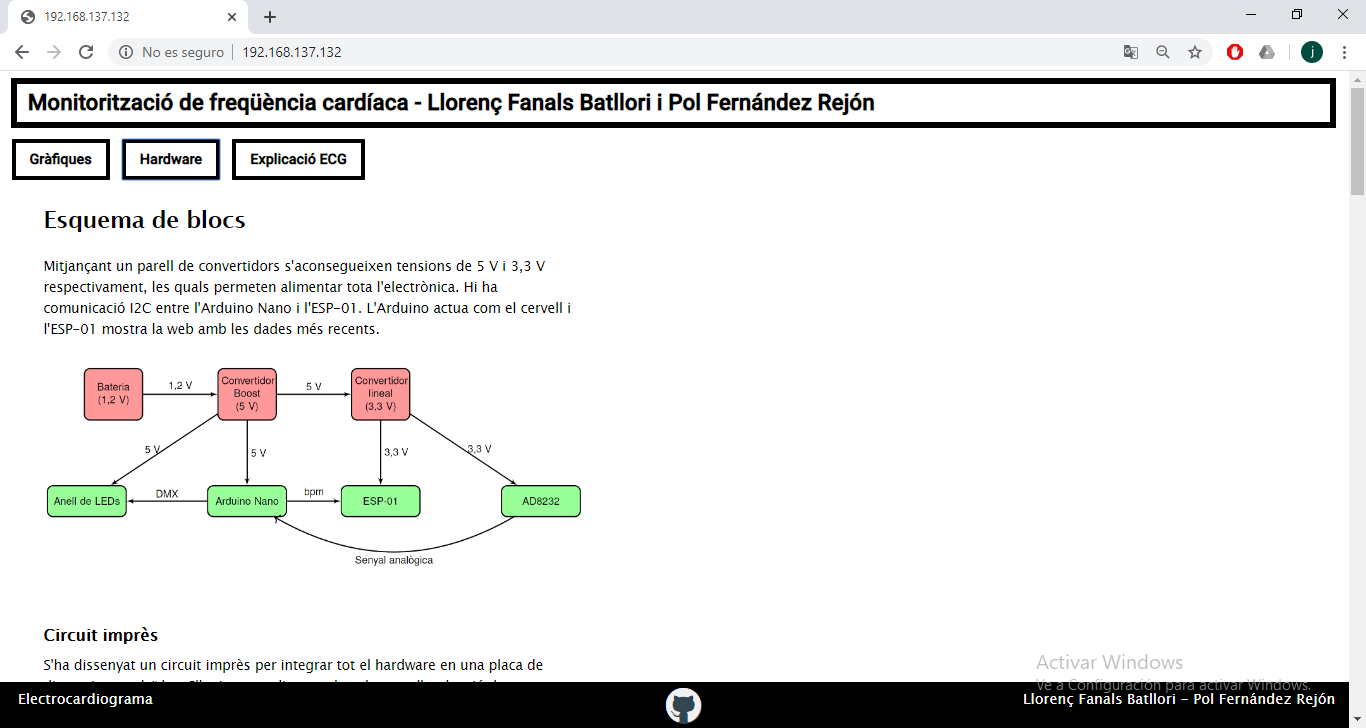
\includegraphics[scale=0.43]{images/web_hardware.png}}
\end{center}
\caption{Apartat de hardware}
\label{fig:2}
\end{figure}







\clearpage


% Table generated by Excel2LaTeX from sheet 'Hoja1'
%\begin{table}[H]
%  \centering
%    \begin{tabularx} {\textwidth} {|X|r|} \hline
%  \multicolumn{1}{|c|}{Descripció} &  \multicolumn{1}{c|}{Quantitat}\\ \hline \hline
%
 %   Placa GLC 330 W & 10 \\ \hline
%    Inversor FRONIUS Primo 3.0-1 Light 3kW & 1 \\ \hline
%    Metres cable Ethernet RJ-45 CAT 8 & 10 \\ \hline
%    Metres cable 4 m$m^2$ PVC & 45 \\ \hline
 %   Metres cable 1,5 m$m^2$ PVC & 100 \\ \hline
 %   Punteres Enghofer E 4-10, 4 m$m^2$, 10 mm & 20 \\ \hline
 %   Punteres Enghofer E 1.5-10 1,5 m$m^2$ 10 mm & 12 \\ \hline
 %   Cinta aïllant 10 m 1,6 cm & 3 \\ \hline
 %   Caixa estanca Solera CONS 100x100x55 mm & 2 \\ \hline
  %  Canal Euroquint 25,16 mm 1,5 metres & 20 \\ \hline
%    Curva canal VECAMCO & 10 \\ \hline
%    Paquet de 50 brides 200x2,6  mm & 2 \\ \hline
%    Regleta nylon 12 pols 16 mm & 4 \\ \hline
%    Premsaestopes M12 & 10 \\ \hline
%    Cargol autoroscant M4 16 mm & 12 \\ \hline
%    Tacs Fischer 072095 nylon 6x50 mm & 50 \\ \hline
%    Díode SM74611KTTR & 10 \\ \hline
%            Hores enginyer & 1 \\ \hline
%    Hores oficial de primera & 12 \\ \hline
%    Hores oficial de segona & 12 \\ \hline
%    \end{tabularx}%
%  \label{tab:addlabel}%
% \end{table}%
